\section{Business processes}
	In this section we'll provide BPMN-models \cite{bpmn} of todays work processes, and show how these work processes will benefit from our system. There might be inaccuracies in 
    the models, but to our knowledge there isn't any major flaws. Due to the fact that most of the users of today's system are students this is the perspective we've focused on in this project. It's worth nothing that all staff should benefit from the new system.

\subsection{Registering for a subject or course}
	As shown in Figure \ref{fig:Register-old}, the current process of finding, selecting and registering for courses is very cumbersome for the students.
The information about each course is spread around on different sites, and due to It's Learning being used to handle most of the information released during a semester,
there is no simple way for students to see what a course actually contains.

Figure \ref{fig:Register-new} shows our suggested changes to this process.
With all information gathered at a single location, we can offer students a coherent experience and improved functionality.
The students can follow the old approach, and manually look through courses, log in at the end, and register,
or they can at any earlier point choose to log in and utilize the course suggestion feature to simplify selection. It's worth nothing that even though the work-flow can seem a bit similar in certain cases, the intention is that this information should be more accessible and more correct than today.\\ 
\begin{figure}[H]
    \centering
    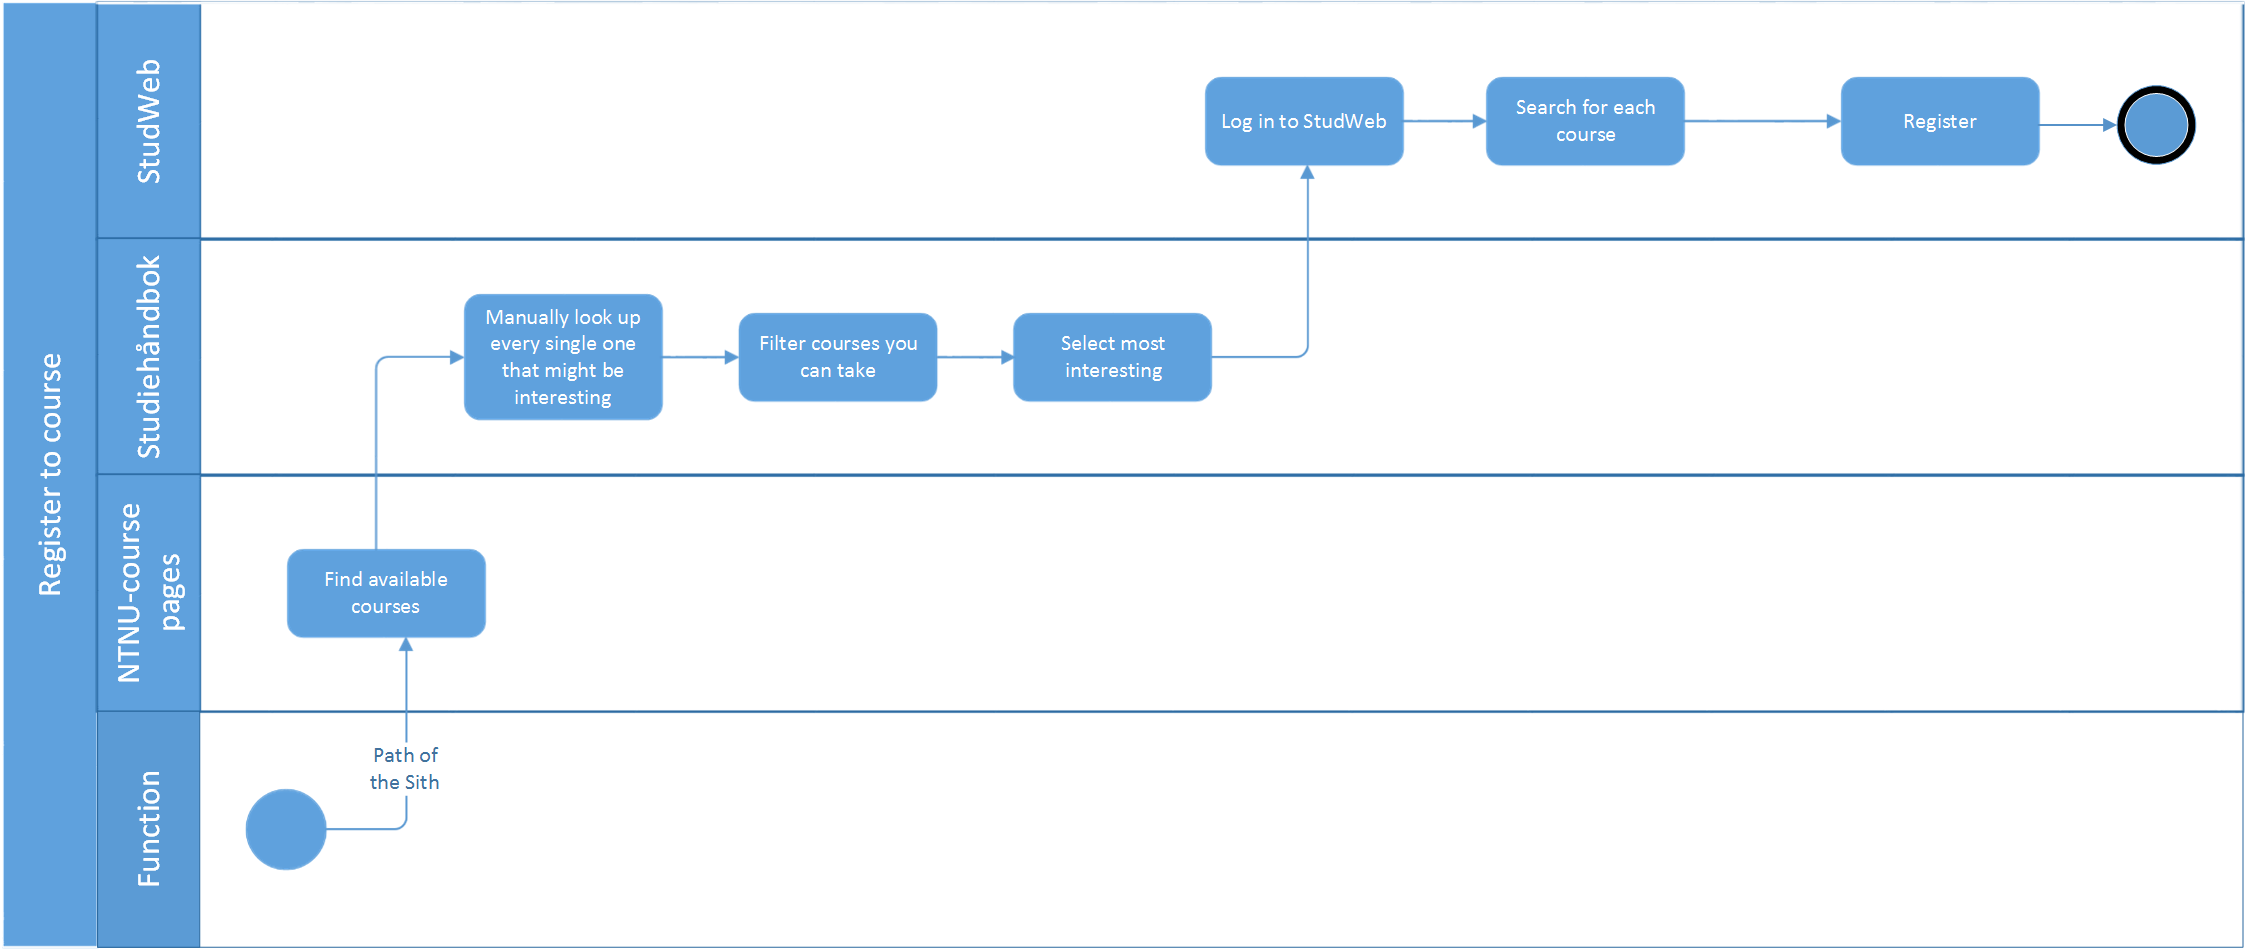
\includegraphics[width=\textheight, angle=-90]{BPMN-register-old}%apparently sets width first and then rotates
    \caption{Model of the current process of registering for a course.}
    \label{fig:Register-old}
\end{figure}
\noindent
Course suggestion works by the system comparing the available subjects to the ones you've already taken, if there are subjects in which your results were good the system will
suggest subjects that are close to, or in the same field as those subjects. It will also filter out any courses for which you might be missing pre-requesits.\\

\noindent
One of the complaints against It's Learning is that all courses are locked so that only students following the course can get access to the information. This has led to a 
fragmentation between courses using It's Learning to provide the students with information and resources, and the courses which provide their own website. Our system will allow staff
to choose wether or not a subject should be publicly available or not. Using discretionary access controls staff can also create certain pages, folders or files that aren't accessible for people not following (or not logged in). This granulary access control would provide opportunity to streamline and provide a uniform experience across subjects and diciplines. The BPMN-model for choosing course does not reflect these abilities since it does not affect the process, only how much information is available to the students. 

\begin{figure}[H]
    \centering
    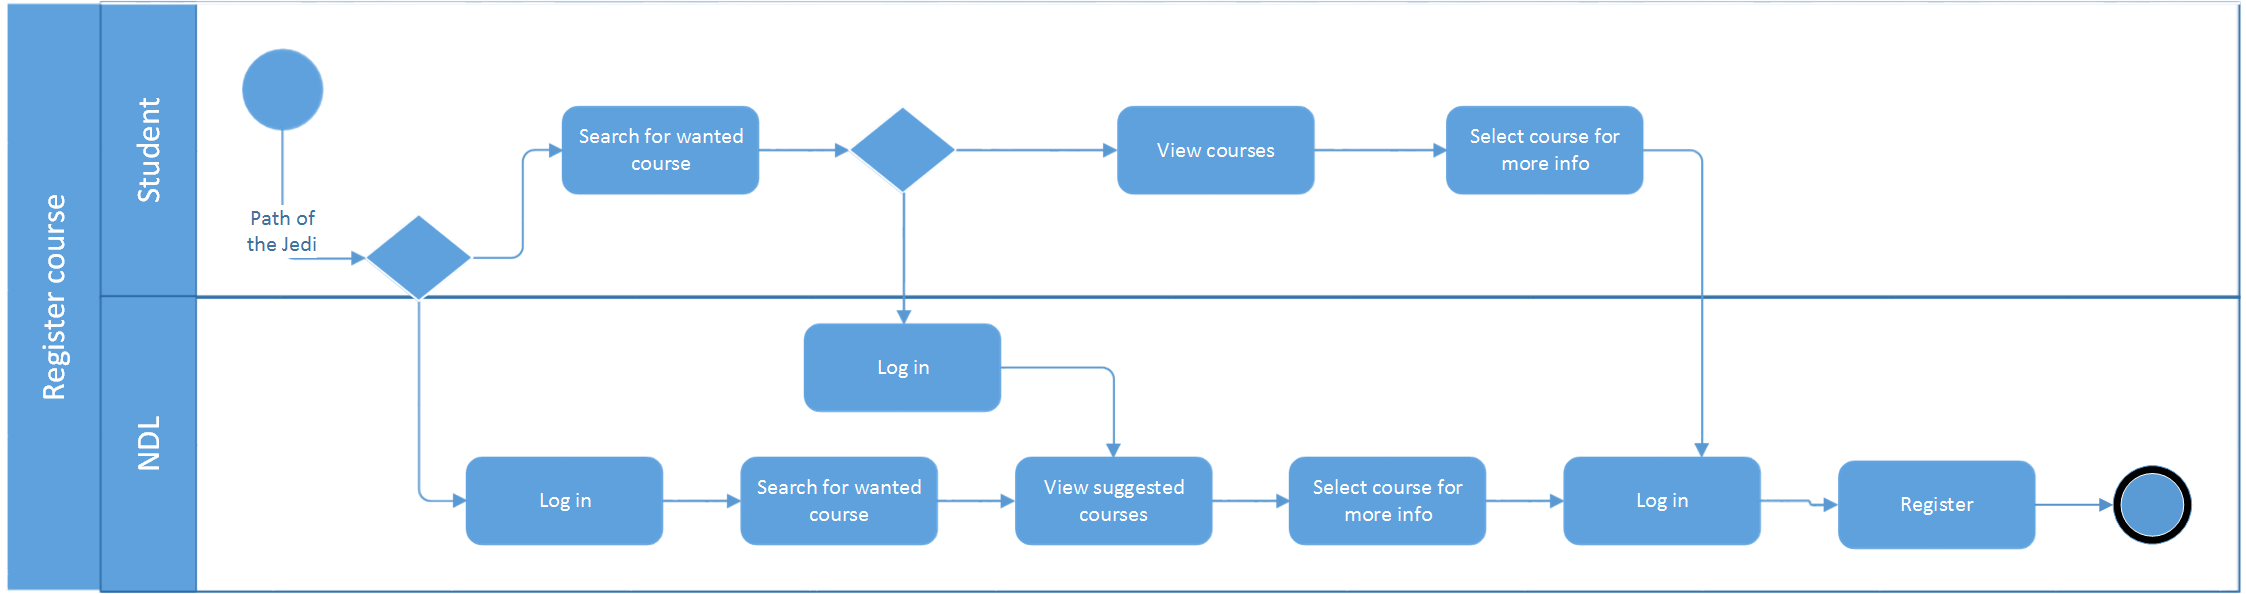
\includegraphics[width=\textheight, angle=-90]{BPMN-register}
    \caption{How we envision our new process of registering for a course should be.}
    \label{fig:Register-new}
\end{figure}

\subsection{Complaining on a grade}
	The current complaint-process, illustrated in Figure \ref{fig:Complain-old}, is split across several systems, and forces most students to file complaints in writing,
which are later digitized, slowing the process down unnecessarily. Our proposal is to completely digitize this process by allowing the complaint to be delivered electronically,
as well as unifying the different sites included in the process as shown in Figure \ref{fig:Complain-new}.\\

\begin{figure}[H]
    \centering
    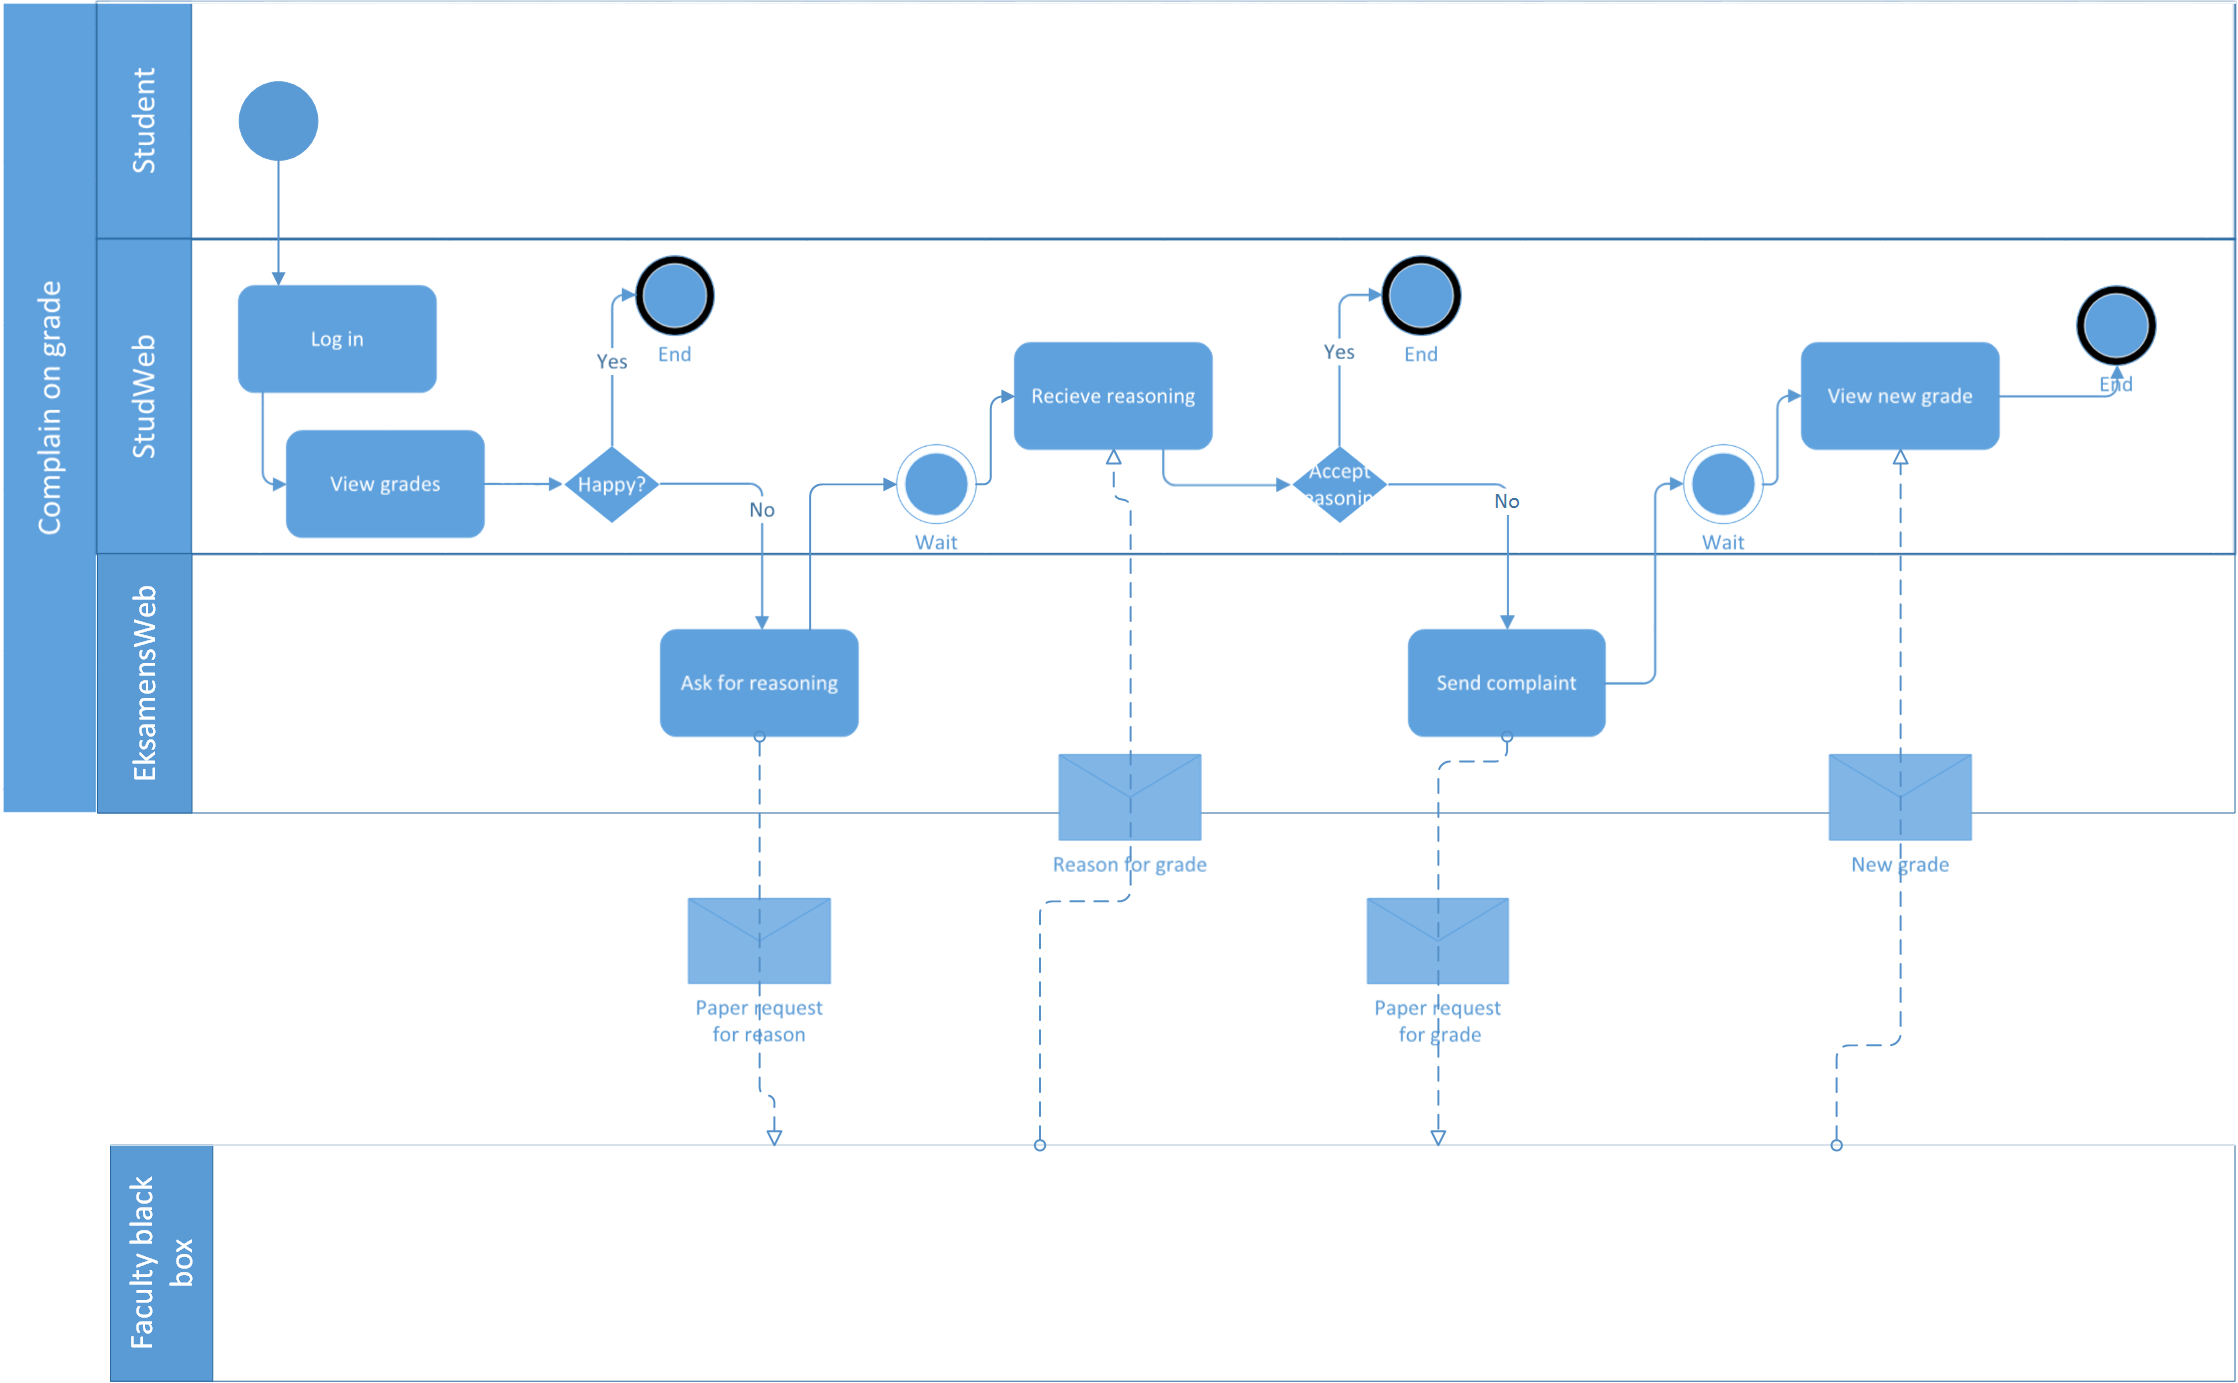
\includegraphics[width=\textheight, angle=-90]{BPMN-Complain-old}
    \caption{A simplified model of the current process of complaining on a grade.}
    \label{fig:Complain-old}
\end{figure}
\noindent
Behind the curtains NUDL would be registering dates and times, making sure that everything happens at the right time (or that a student isn't allowed to complain after the deadline). One possible feature could be to collect anonymized data for statistical purposes and use this to look for areas of improvement.

\begin{figure}[H]
    \centering
    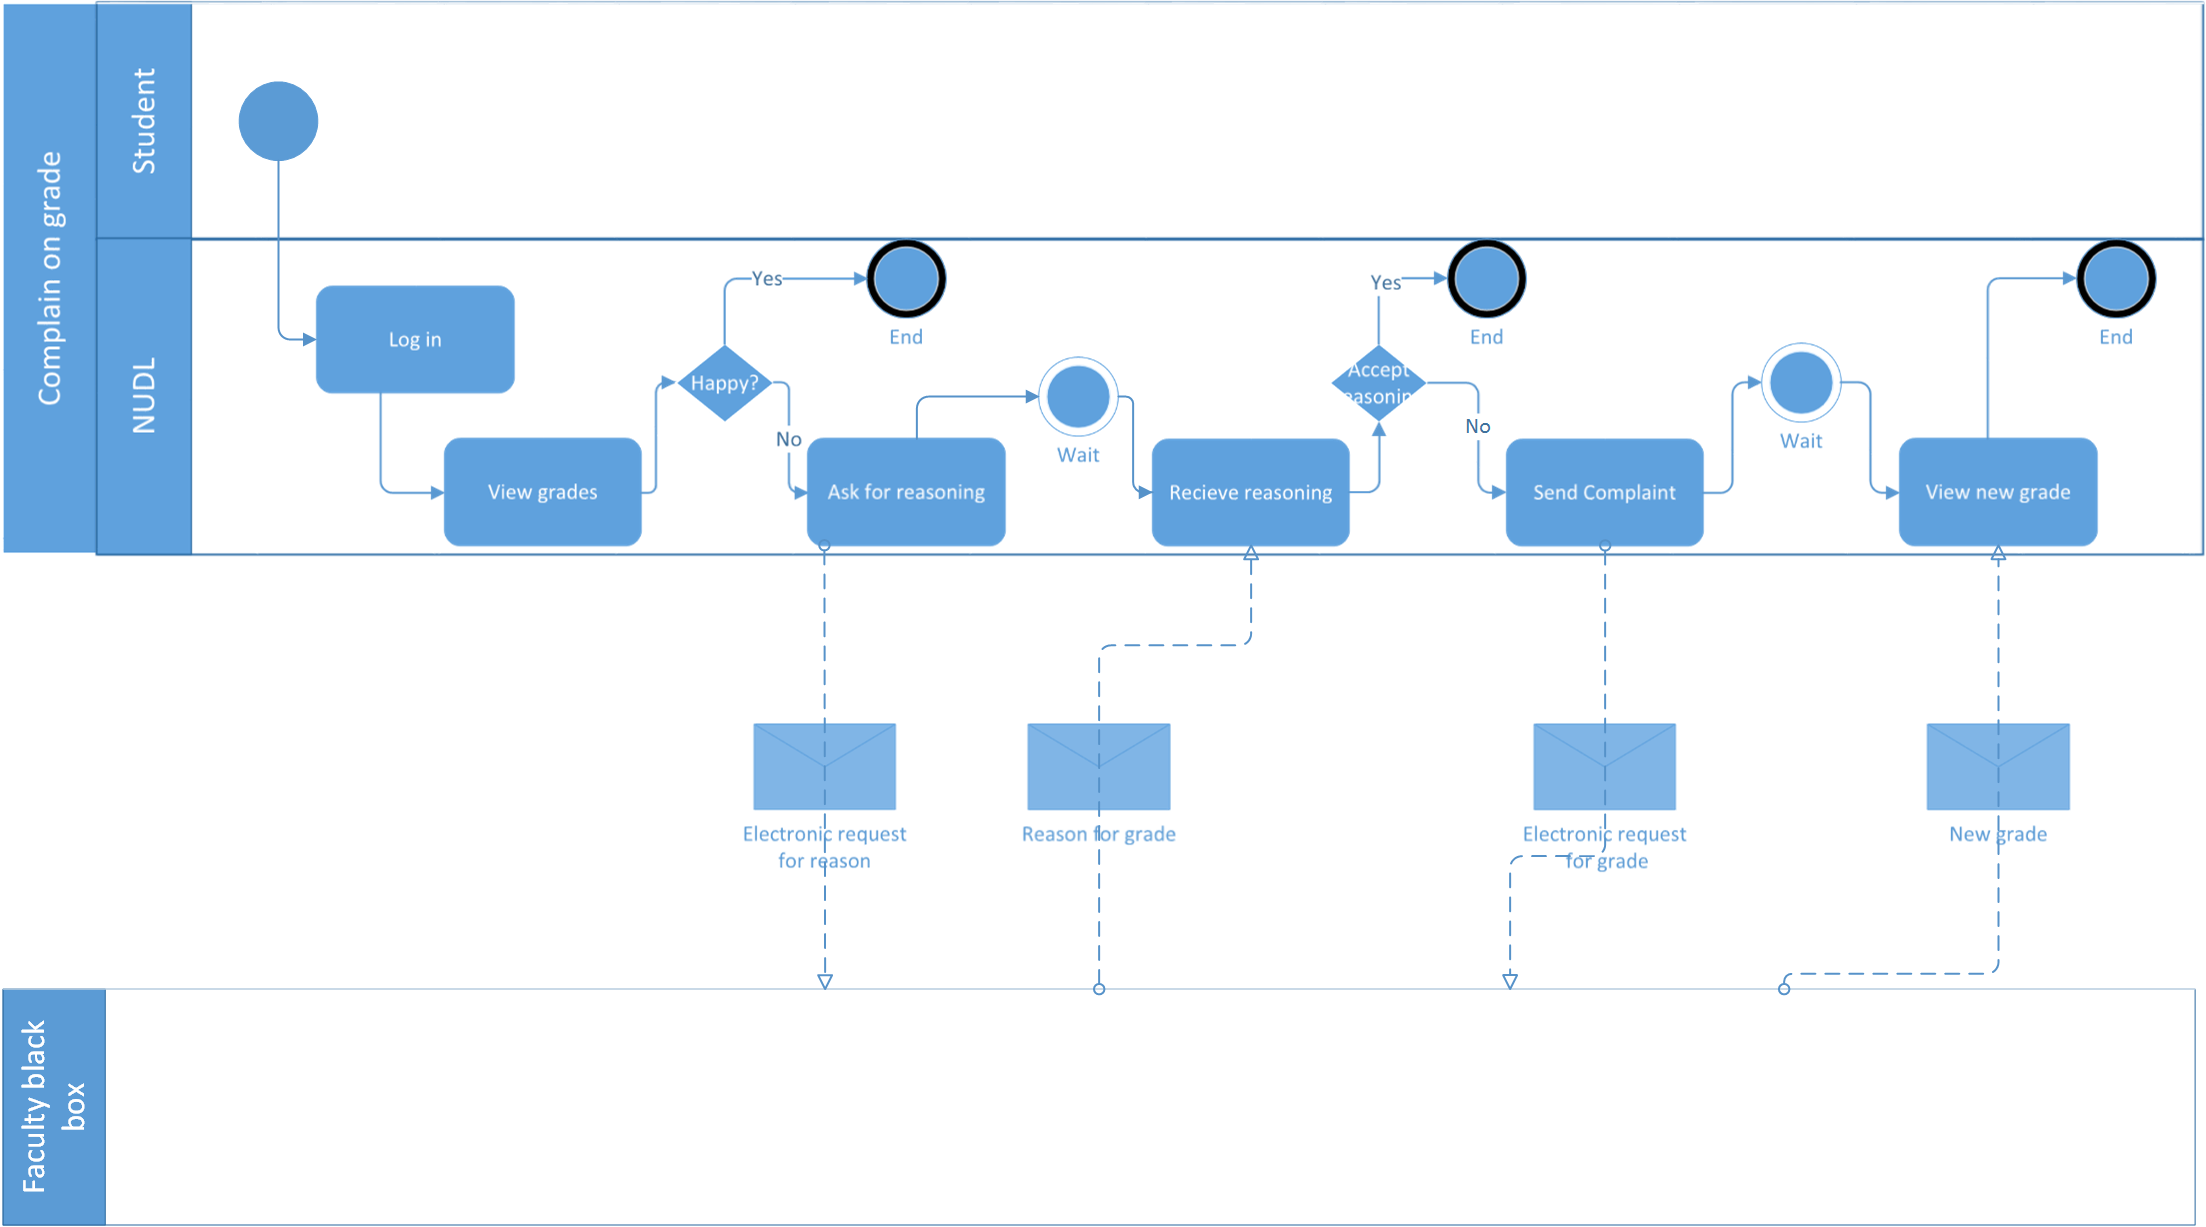
\includegraphics[width=\textheight, angle=-90]{BPMN-Complain}
    \caption{How we envision the new process of registering a complaint should be.}
    \label{fig:Complain-new}
\end{figure}
